\documentclass[11pt, twocolumn]{article}
\usepackage[utf8]{inputenc}
\usepackage[a4paper, margin=2cm]{geometry}
\usepackage[portuguese]{babel}
\usepackage{multicol}
\usepackage{graphicx}
\usepackage{tabularx}
\usepackage{abstract}
\begin{document}
\title{Relátio referente a construção do processador SAP1 em Python}
\author{Bruno Gomes}
\date{\today}
\twocolumn[
\maketitle
\begin{onecolabstract}
  Foi construído um processador virtual em Python que segue a arquitetura SAP1. Primeiramente foi criado um pacote em Python capaz de simular circuitos digitais e em seguida foi implementado uma micro-arquitetura conhecida para o SAP1. O processador foi testado e foi usado para rodar programas escritos em linguagem de maquína.
\end{onecolabstract} ]
\section{Introdução}

\subsection{Arquitetura}
   A arquitetura SAP1 é uma arquitetura de 8 bits com um conjunto de instruções minimo, essa arquitetura é apresentada por Malvino. A figura \ref{fig-blocks} é um diagrama de blocos da arquitetura, nota-se dois registradores conectados ao somador, um registrador de saida, banco de memória 4x8 bits e os demais componentes experados como MAR, PC, CU. Todos os blocos de comunicam atraves de uma bus central (bus W), para que isso seja possível as saídas dos blocos devem usar lógica de três estados. O conjunto de instruções da arquitetura é apresentado na tabela \ref{tab-inst}, essas instruções são: ADD, LDA, SUB, HLT e OUT (a instrução OUT é omitida na construção do processador virtual). Percebe-se que essa arquitetura não apresenta nenhuma instrução de jump, o que limita muito o tipo de computação que pode ser feito, porém para fins de aprendizado isso é irrelevante. Todas as instruções seguem o mesmo formato, a palavra de 8 bits é dividade em opcode (4 bits mais siginifactivos) e 4 bits de endereço (4 bits menos significativos).

   \begin{figure}
     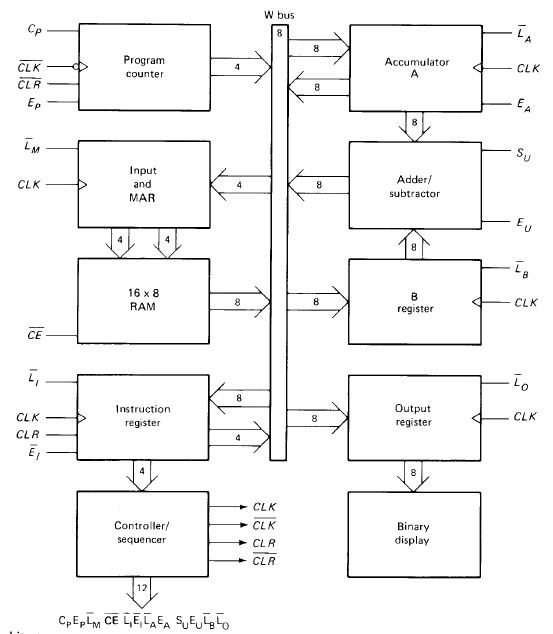
\includegraphics[width=0.5\textwidth]{blocks.jpg}
     \caption{Diagrama de blocos do processador SAP1. (Malvino)}
     \label{fig-blocks}
   \end{figure}
   
\subsection{Micro arquitetura}
A micro arquitetura implementada possui foi baseada na implementação feita na literatura, cada instrução demora 6 ciclos do relógio para serem executadas. A unidade de controle construída recebe como sinal o ciclo da micro-instrução (contador de 0-5 com um comparador para reset) e o op-code da instrução, internamente usa uma memória ROM como uma look-up table e tem como saída as 12 flags que são usadas para controlar os blocos do processador.

\begin{table}
  \caption{Instruções da arquitetura SAP1 e suas descrições.}
\begin{tabular*}{\linewidth}{lcp{8cm}}
  \hline
 Inst. & Op code & Descrição \\
 \hline
 LDA         &     0x0 & Carrega o acumulador com o valor contido no endereço dado. \\
 ADD         &     0x1 & Soma o valor presente no acumulador com o valor contido no endereço dado. \\
 SUB         &     0x2 & Subtrai o valor presente no acumulador com o valor contido no endereço dado.\\
 OUT         &     0xE & Escreve o valor contido no acumulador ao registro de saída (Out). \\ 
 \hline
\end{tabular*}
\label{tab-inst}
\end{table}


\subsection{PDD}
A implementação do processador foi feita usando o programa desenvolvido durante a fase inicial do projeto, a esse programa foi dado o nome PDD que atua como um simulador de circuitos digitais com sinais ideais. PDD é escrito em Python puro e é distribuido como um pacote Python comum. A descrição completa da arquitetura do simulador é complexa e foje do escopo desse artigo porém as principais caractéristicas são instrutivas. PDD foi construído com orientação a objetos em seu núcleo. Novos circuitos são implementados pelo usuário de maneira direta utilizando o conceito de herança. No momento PDD não possui um front-end que seja amigável a usuários inexperientes porém é completamente capaz de simular um processador como será demostrado. PDD dispõe ao usuário os principais circuitos combinacionais, sequenciais e as portas lógicas; a partir desses circuitos pode-se construir qualquer circuito digital.

\section{Procedimento Experimental}
  
A fim de expandir os conceitos de modularidade muito presentes no paradigma de circuitos digitais o processador foi separado em 2 partes que interagem, os blocos CU e SAU. O bloco CU é a unidade de controle do processador e como entrada recebe o ciclo da micro instrução (ic) e o opcode da instrução sendo executada (iw), e como saída a palavra de controle que é aceita pela SAU para controlar os elementos do processador; SAU contém todos os outros elementos descritos anteriormente, SAU recebe um sinal de clock e reset (clk e r) e diversas flags de controle como entrada; como saida o ciclo da micro-instrução (ic), a bus de saída do registrador out e o opcode da intrução (iw). A separação foi feita para facilitar no processo de desenvolvimento do processador pois tendo dois modulos bem definidos como a SAU e CU facilitam imensamente o processo de debugar, algo muito prezado durante o desenvolvimento do PDD. Esse metodo possibilita que cada bloco seja testado com facilidade usando testes unitarios, conceito esse muito comum na programação. A fígura \ref{fig-cu} demonstra os dois blocos e como os mesmos interagem.

Como todo circuito em PDD, foi criado uma classe para o bloco CU com as entradas e saídas como descritas anteriormente. Internamente CU é apenas uma look up table usando uma memoria ROM. O endereço da memoria é dada pela concatenção das buses ic e iw, a memoria tem como tamanho de palavra 12 bits, um bit para cada flag da SAU, as micro instruções do processador estão disponiveis em \cite{malv}. A tabela \ref{tab-flags} lista as 12 flags e suas funções. 

\begin{table}
\begin{tabular}{ll}
\hline
Flag & Descricao \\
\hline
cp & Incrementar PC no proximo clk \\
ep & Tristate de saida do PC \\
lm & Tristate de entrada do MAR \\
ce & Tristate saida da RAM \\
li & Tristate de entrada do IR \\
ei & Tristate de saida do IR \\
la & Tristate de entrada do acumulador \\
ea & Tristate de saida do acumulador \\
su & Flag de subtracao para o adder/subtractor \\
eu & Tristate de saida para o adder/subtractor \\
lb & Tristate de entrada para o registrador B \\
lo & Tristate de entrada para o registrador output \\
\hline
\end{tabular}
\label{tab-flags}
\end{table}

   \begin{figure}
     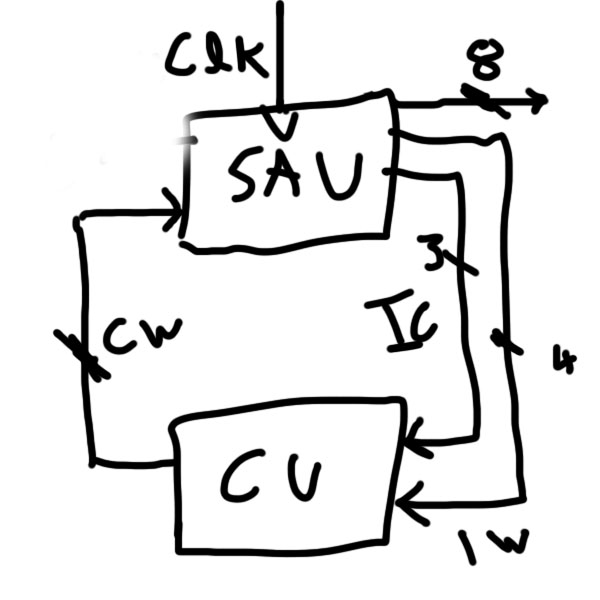
\includegraphics[width=0.5\textwidth]{cu.jpg}
     \caption{Diagrama de blocos ilustrando a conexão entre SAU e CU. Os sinais iw e ic são o op-code da instrução e o ciclo da micro-instrução, respectivamente, cw é a palavra de controle com as 12 flags referente aos blocos em SAU. Nota-se uma bus de saída em SAU de tamanho 8 referente ao registrador OUT.}
     \label{fig-cu}
   \end{figure}
 
O bloco SAU foi implementado da mesma maneira como pode ser visto na imagem \ref{fig-blocks} com a adição de um contador e um comparador que são responsáveis por marcar o ciclo das micro instruções, o comparador tem como uma das entradas o sinal $0x5$ e na outra o contador, sua saída é ligada à entrada de reset "r" do circuito contador.

Finalmente uma ultima classe referente ao processador foi criada. O processador tem duas entradas: reset (r) e clock (clk) e uma unica saída chamda de out. Internamente o processador é composto pelos blocos SAU e CU. As flags de SAU são conectadas a partir de CU os sinais r e clk do processador, as saidas iw e ic são ligadas ao bloco CU. Tendo feito essas conexões a construção do processador está finalizada.

Para executar programas no processador basta escrever em um arquivo de texto o conteúdo da memória e usar o método "fburn" da class ROM para carregar o programa. Feito isso basta gerar pulsos de clock utilisando os comandos existentes para operar sobre a bus clk do processador.

\section{Resultados}

Foram escritos 3 programas para o programa executar. Os programas foram executados e foi inspecionado se o resultado escrito para o registrador "out" era o esperado.

\subsection{Programa 1}
O primeiro programa escrito simplemeste carrega um valor no registrador ACC com a instrução LDA e move esse valor para o registrador out com a instrução OUT. Este programa é extremamente simples e foi usado para testar as intruções básicas. A tabela \ref{tab-p1} contém o contéudo escrito na memória do processador. O resultado esperado da execução do programa é que o valor no registrador out seja 3 e o resultado obtido está de acordo.

\begin{table}
  \caption{Palavras na memória para execuçao do programa 1}
\begin{tabular}{ll}
  \hline
  Endereço & mem. Conteudo \\
  \hline
  0x0 & 0x0F \\
  0x1 & 0xE0 \\
  0x2 - 0xE & 0x0 \\
  0xF & 0x03 \\
  \hline
  \end{tabular}
\label{tab-p1}
\end{table}

\subsection{Programa 2}
O programa 2 testa que a instruçao de addição. O valor do inicial do acumulador (0) é somado ao valor presente do endereço 0xF (valor 3), em seguida o valor presente no acumulador (3) é escrito no registrador de saída. O resultado obtido foi $3$, como esperado.

\begin{table}
  \caption{Palavras na memória para execuçao do programa 2.}
\begin{tabular}{ll}
  \hline
  Endereço mem. & Conteudo \\
  \hline
  0x0 & 0x1F \\
  0x1 & 0xE0 \\
  0x2 - 0xE & 0x0 \\
  0xF & 0x03 \\
  \hline
  \end{tabular}
\label{tab-p2}
\end{table}

\subsection{Programa 3}
O terceiro e ultímo programa executado utiliza as intruções LDA, OUT e ADD que foram testadas individualmentes e combina-as em um uníco programa utilizando todas as instruções do processador. Primeiramente o valor 3 é carregado no acumulador, em seguida é somado 6 ao valor no acumulador, subtrai-se 2 do valor e finalmente o resultado é escrito no registrador OUT. O resultado obtido foi 7, demonstrando que o processador está executando todas as intruções corretamente.

\begin{table}
  \caption{Palavras na memória para execuçao do programa 3}
\begin{tabular}{ll}
  \hline
  Endereço mem. & Conteudo \\
  \hline
  0x0 & 0x0F \\
  0x1 & 0x1E \\
  0x2 & 0x2D \\
  0x3 & 0xE0 \\
  0x4 - 0xC & 0x0 \\
  0xD & 0x02 \\
  0xE & 0x06 \\
  0xF & 0x03 \\
  \hline
  \end{tabular}
\end{table}
\label{tab-p3}


\section{Conlusão}

A ferramenta PDD possibilita a simulação de circuitos digitais e foi utilizado para replicar a arquitetura descrita na literatura. A arquitetura escolhida é simples porém a base de qualquer arquitetura está presente nela, sendo assim é possivel utilizar a mesma ferramenta para simular uma arquitetura mais completa (mais instruções) e diferentes tamanhos de palavras. O objetivo da ferramente construida é respeitar os principios dos circuitos digitais, gerar uma abstração que seja familiar para estudantes com expêriencia em montar circuitos em protoboards e possibilitar a construção de circuitos digitais abstratos usando os principios da programação orientada a objetos.

Um grande defeito de PDD é velocidade, devido à estrutura dada ao aplicativo pode-se notar uma performance que se deixa a desejar. Para corrigir esses problema existem varias alternativas como: utilizar caches para reduzir redundância devido aos eventos, utilizar algoritimos mais sofisticados e paralelismo para realizar as operações e trocar a pureza da implementação dos blocos sequências e combinacionais (devido ao fato de terem sido utilizados somentes portas lógicas para a sua construção) e optar por uma implementação rápida utilizando as operações já construidas no processador do usuário.

\end{document}
